\section{Implementação do Algoritmo Morpheus}
\label{sec:7.2}

No Morpheus, a execução do algoritmo genético ocorre principalmente na classe GradeService, responsável por receber os dados acadêmicos, organizar as estruturas internas de processamento, gerar a população inicial, aplicar os operadores evolutivos e retornar a melhor grade horária encontrada. A entrada principal do algoritmo é uma requisição do tipo GradeRequest, composta por disponibilidades docentes, matrizes curriculares, turmas, vínculos entre professores e disciplinas, parâmetros do algoritmo genético e parâmetros da função \textit{fitness}.

A obtenção dos dados pode ocorrer por meio de uma camada externa ao algoritmo, responsável por consultar o banco de dados e montar a estrutura de entrada. No arquivo data\_service.py, são buscadas disponibilidades, matrizes, turmas e vínculos entre usuários e disciplinas. Entretanto, a execução do algoritmo genético em si não realiza consultas diretas ao banco: o GradeService recebe uma requisição já estruturada, constrói seus índices e caches em memória e, a partir dessas informações, executa o processo evolutivo.

Antes de iniciar a evolução, o Morpheus constrói índices em memória por meio do método \_construir\_indices. Essa etapa transforma as listas recebidas na requisição em estruturas de acesso rápido, criando mapas para recuperar disponibilidades, matrizes e turmas por seus identificadores, além de caches que relacionam disciplinas aos professores habilitados, turnos às disponibilidades e associações entre matrizes, turmas e turnos. Entre essas estruturas, destaca-se o cache de candidatos por matriz: para cada matriz curricular, o algoritmo identifica quais disponibilidades podem ser utilizadas, considerando o turno da turma e o vínculo entre professor e disciplina.

A representação genética do Morpheus utiliza explicitamente uma dataclass chamada Gene, com dois campos: matriz\_id e disponibilidade\_id. O cromossomo, formado por uma lista de genes, corresponde a uma grade horária candidata completa. Além da classe Gene, o Morpheus define a dataclass Individuo, que armazena o cromossomo e sua respectiva \textit{fitness}, e a dataclass Metricas, que concentra informações como quantidade de erros, conflitos, disciplinas não alocadas e dados inválidos. Quando uma matriz não possui candidatos válidos, o Morpheus utiliza o valor ID\_NAO\_ALOCADO = 0.

A população inicial é gerada pelo método \_inicializar\_populacao, que cria cromossomos por meio do método \_gerar\_cromossomo. Para cada matriz, o algoritmo verifica se existem turno, disciplina e turma associados e consulta a lista de candidatos válidos previamente construída. Caso existam candidatos, o algoritmo escolhe aleatoriamente uma disponibilidade, tentando priorizar aquelas que ainda não geram colisão para a mesma turma no mesmo dia e turno. Essa estratégia pode ser classificada como uma inicialização aleatória guiada por restrições.

A função \textit{fitness} é implementada no método \_calcular\_fitness. A avaliação começa com uma pontuação base proporcional ao tamanho do cromossomo, acrescida de bônus por alocações válidas e bônus de diversidade. As penalidades são os elementos mais decisivos: genes não alocados recebem penalidade padrão de 10.000 pontos; conflitos de professor recebem 12.000 pontos, por serem considerados os mais críticos; conflitos de turma recebem 8.000 pontos; dados inválidos recebem 10.000 pontos. Essa hierarquia de pesos demonstra uma priorização interna da implementação.

A evolução da população ocorre por meio do método \_evoluir\_populacao, que combina elitismo, seleção por torneio com \textit{crossover} de um ponto, mutação gene a gene, melhoria local e reparo inteligente. O \textit{crossover} de um ponto sorteia uma posição de corte no cromossomo, de modo que o primeiro filho recebe os genes iniciais do primeiro pai e os genes finais do segundo. A mutação é guiada por restrições do domínio, selecionando a nova disponibilidade dentro do conjunto de candidatos válidos da matriz correspondente.

Uma característica própria do Morpheus é a existência de uma etapa explícita de melhoria local antes do reparo inteligente. Após a mutação, o método \_melhorar\_alocacoes\_locais percorre o cromossomo buscando genes não alocados e tenta encontrar um candidato capaz de preencher a lacuna com pontuação interna de conflito igual a zero. Em seguida, o método \_reparar\_inteligente percorre o cromossomo em até duas passagens, identificando genes problemáticos e buscando o melhor candidato dentro das disponibilidades válidas por meio de uma pontuação interna de conflito. Quando encontra uma opção sem conflito, realiza a substituição; quando não há solução perfeita, pode aceitar uma melhoria parcial.

O critério de parada do Morpheus combina um limite fixo de gerações com mecanismos de parada antecipada. A execução pode ser interrompida quando uma solução sem erros é encontrada, isto é, quando a melhor grade da geração possui quantidade total de erros igual a zero. Na implementação, esse total corresponde à soma entre disciplinas não alocadas, conflitos de professor, conflitos de turma e dados inválidos ou incompletos. Quando essa condição ocorre, a geração da solução sem erros é registrada e o processo evolutivo é encerrado imediatamente.

Além disso, o Morpheus interrompe a evolução quando passa muitas gerações sem melhorar a melhor \textit{fitness} global. O limite de gerações sem melhoria é calculado como 20\% do total de gerações configurado, respeitando um mínimo de 25 e um máximo de 200 gerações, conforme a expressão \texttt{max(25, min(200, numeroGeracoes * 0.20))}. Assim, para 100 gerações configuradas, o limite sem melhoria é 25; para 1.000 gerações, é 200; e para 2.000 gerações, permanece em 200. A melhora considerada nesse critério é uma melhora de \textit{fitness}, não apenas uma redução direta da quantidade de erros. Caso a diferença entre a geração atual e a última geração com melhora alcance esse limite, a execução é interrompida e a resposta indica parada antecipada.

Por fim, se nenhuma das condições anteriores for satisfeita, o algoritmo continua até atingir o número máximo de gerações configurado. O valor padrão utilizado pelo Morpheus é de 1.000 gerações, podendo ser sobrescrito na requisição por meio do parâmetro \texttt{numeroGeracoes}. Ao final, o melhor cromossomo é decodificado pelo método \_decodificar\_cromossomo e as métricas finais são calculadas pelo método \_calcular\_metricas\_detalhadas.


\begin{figure}[H]
\centering
\caption{Fluxo de execução do algoritmo genético Morpheus}
\label{fig:fluxo-morpheus}

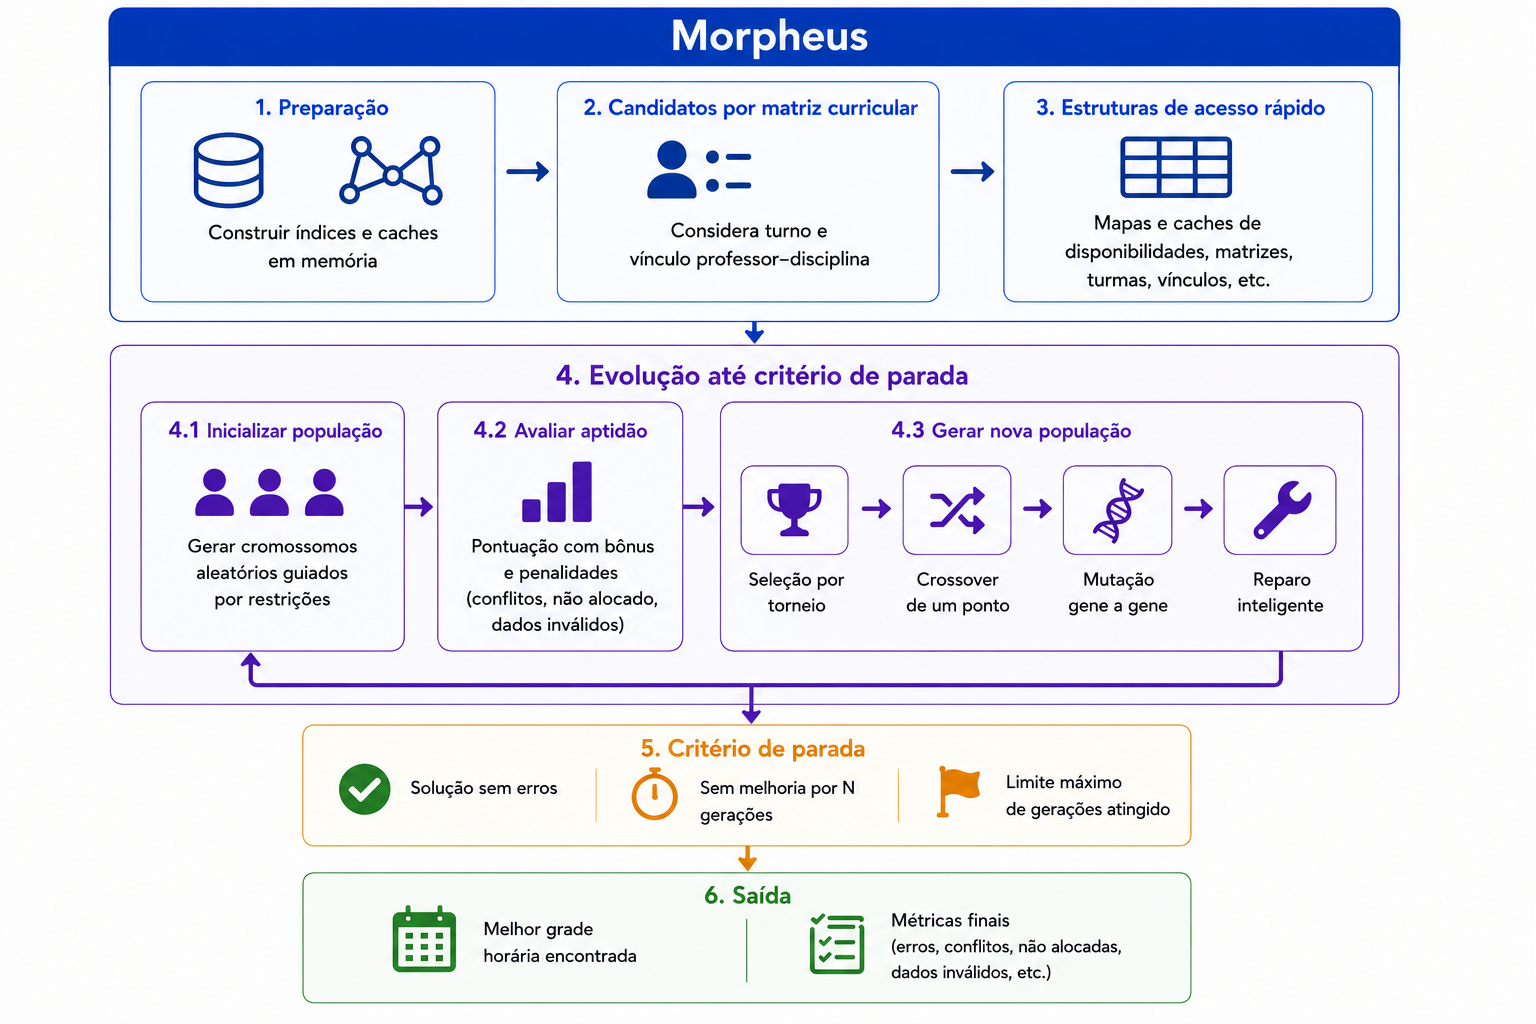
\includegraphics[width=0.85\textwidth]{figuras/Figura_16_ilustracaoFluxoMorpheus.png}

\vspace{0.2cm}
\fonteautores
\end{figure}
